% M.Tech thesis — assembled 2026-07-12 from the tinker-rl-lab research program.
% Chapter <- paper provenance map: see Appendix A (all 17 program documents).
\documentclass[12pt,a4paper,oneside]{report}

\usepackage[margin=1in]{geometry}
\usepackage{amsmath,amssymb,amsthm}
\usepackage{booktabs}
\usepackage{graphicx}
\usepackage{enumitem}
\usepackage[hidelinks]{hyperref}
\usepackage{xcolor}
\usepackage{tikz}
\usetikzlibrary{arrows.meta,positioning,shapes.geometric,decorations.pathreplacing}
\usepackage{pgfplots}
\pgfplotsset{compat=1.18}
\usepackage{setspace}
\onehalfspacing

\newcommand{\ZVF}{\ensuremath{\mathrm{ZVF}}}
\newcommand{\GU}{\ensuremath{\mathrm{GU}}}
\newtheorem{theorem}{Theorem}
\newtheorem{lemma}{Lemma}
\newtheorem{definition}{Definition}

\title{The Zero-Variance Fraction:\\
Diagnosing and Budgeting Signal Starvation in\\
Group-Relative Reinforcement Learning Post-Training\\
of Large Language Models}
\author{Arvind C R}
\date{July 2026}

\begin{document}

% ---------------- Front matter ----------------
\begin{titlepage}
\centering
{\Large \textbf{The Zero-Variance Fraction: Diagnosing and Budgeting Signal
Starvation in Group-Relative Reinforcement Learning Post-Training of Large
Language Models}}\\[2cm]
A thesis submitted in partial fulfilment of the requirements for the degree of\\[0.3cm]
{\large \textbf{Master of Technology}}\\[1.5cm]
by\\[0.3cm]
{\large \textbf{Arvind C R}}\\[1.5cm]
Under the guidance of\\[0.3cm]
{\large Prof.\ Ramesh Prakash Guledgudd}\\[2cm]
{\large PES University}\\[0.3cm]
July 2026
\end{titlepage}

\chapter*{Declaration}
I declare that this thesis presents my own work, carried out in the fourth
(solo) semester of the M.Tech programme as a continuation of the Group~6
capstone project of semester three. All experimental artifacts --- run
manifests, result files, analysis scripts, and the seventeen working papers
this thesis consolidates --- are version-controlled in the public repository
\texttt{arvindcr4/tinker-rl-lab}, with provenance boundaries between the group
and solo phases recorded in \texttt{PROJECT\_HISTORY.md}. Work that used
AI-assisted drafting is identified as such in Chapter~9; every quantitative
claim in this thesis traces to a named artifact.

\chapter*{Abstract}
Group-relative policy optimisation (GRPO) trains language models on groups of
$G$ completions per prompt, with each completion's advantage computed relative
to its group. Under binary verifiable rewards, any group whose completions all
receive the same reward --- all correct or all incorrect --- contributes
exactly zero gradient. This thesis studies the fraction of such groups, the
\emph{Zero-Variance Fraction} (\ZVF{}), as a first-class training signal.

The thesis defends two bounded claims. \textbf{Claim 1:} \ZVF{}, read together
with mean reward, is a cheap online diagnostic that identifies
\emph{zero-advantage regimes} which reward curves alone cannot reveal ---
including the regime where training looks maximally successful (reward
$\approx 1.0$) while every update carries no signal. \textbf{Claim 2:} at a
matched rollout budget on Qwen3-8B/GSM8K, group size controls \emph{which end}
of training starves: $G{=}2$ arms end in a sustained all-correct zero-variance
wall ($\ZVF \approx 0.75$--$1.0$ at reward $\approx 1.0$) while $G{=}16$ arms
hold $\ZVF \le 0.25$ throughout (two seeds per arm). Supporting results
include a calibrated confidence interval for \ZVF{} (Wilson, coverage
0.95--0.98 in all tested settings), a waiting-time reliability budget that
matches observed quantiles at ratio 1.00 across six difficulty strata, and a
six-arm uncapped panel showing no completion-length inflation and no late-\ZVF{}
separation between GRPO and Dr.GRPO at this scale.

The thesis states its non-claims with equal precision: no predictive or causal
power is claimed for \ZVF{} beyond diagnosis; no data-dependent optimal group
size is claimed (the signal-per-rollout objective's optimum is shown to be the
universal $G^\star \in \{2,3\}$ for every difficulty prior --- an algebraic
identity, not an empirical discovery); no adaptive-controller efficacy is
claimed pending a pre-registered compute-matched comparison; and no
generalisation beyond the studied stack (Qwen3-8B, GSM8K-family tasks, a
managed LoRA-only training API) is asserted. A reproducibility chapter turns
the program's own instrumentation failure --- a documented-but-unwired loss
flag that silently made a six-arm GRPO-vs-Dr.GRPO comparison train a single
objective --- into a case study and an eight-item minimum-reportable-stack
standard with a machine-readable registry.

\tableofcontents

% ---------------- Chapters ----------------
% Provenance: P2 abstract/intro, main_zvf.tex framing, advisor brief 2026-07-12,
% consolidation plan v3 claim contract.
\chapter{Introduction}
\label{ch:intro}

\section{The problem: silent signal starvation}
Reinforcement learning from verifiable rewards has become the standard second
stage of language-model training for reasoning tasks. The dominant family of
methods --- GRPO and its variants --- avoids a learned critic by sampling a
\emph{group} of $G$ completions per prompt and centring each completion's
reward against its group mean. This design has a structural blind spot: when
every completion in a group receives the same reward, the centred advantages
are identically zero and the group contributes \emph{no gradient}. Under
binary rewards this happens in exactly two situations --- the model fails
every attempt (too hard) or solves every attempt (mastered). Both ends of
training are therefore starved of signal, and, critically, the second kind of
starvation is invisible in the reward curve: mean reward reads ``success''
precisely while learning has stopped.

This thesis names, measures, calibrates, and budgets that phenomenon through a
single statistic:

\begin{definition}[Zero-Variance Fraction]
At training step $t$, with prompt set $\mathcal{P}_t$ and $G$ completions per
prompt,
\[
\ZVF_t \;=\; \frac{1}{|\mathcal{P}_t|}\sum_{p\in\mathcal{P}_t}
\mathbf{1}\!\left[\operatorname{Var}_{c\sim\mathcal{C}(p)} r(c) = 0\right],
\qquad \GU_t \;=\; 1-\ZVF_t ,
\]
the fraction of groups carrying zero advantage, and its complement, the
fraction of groups carrying usable gradient signal (\emph{gradient
utilisation}).
\end{definition}

\section{Claim contract}
\label{sec:claims}
Following an external adversarial review of this program (Chapter~9), the
thesis is organised around an explicit contract separating what the evidence
supports from what it does not.

\paragraph{Claim 1 (supported; Chapters 4--5).} \ZVF{}, read together with
mean reward, is a near-zero-cost online diagnostic that identifies
zero-advantage regimes. \ZVF{} alone aliases mastery with incapacity; the
reward coordinate disambiguates. Its estimator admits a calibrated confidence
interval (Wilson; empirical coverage 0.95--0.98 in all tested settings), and a
geometric waiting-time model built on it yields a \emph{reliability budget} ---
the $(1{-}\delta)$-quantile of rollouts until the next informative group ---
that matched observed quantiles at ratio 1.00 across six difficulty strata.

\paragraph{Claim 2 (supported; Chapter 6).} At a matched budget of 2{,}560
rollouts per arm on Qwen3-8B/GSM8K (LoRA rank 4), $G{=}2\times160$ steps and
$G{=}16\times20$ steps reach comparable final train reward, but every $G{=}2$
arm terminates inside the all-correct zero-variance wall
($\ZVF\approx0.75$--$1.0$ at reward $\approx1.0$) while $G{=}16$ arms hold
$\ZVF\le0.25$ throughout (seeds 123/456). Group size controls \emph{which end
of training starves}; it is a schedule question, not a constant.

\paragraph{Non-claims (explicit).}
\begin{enumerate}[leftmargin=1.6em,itemsep=1pt]
  \item No predictive or causal power is claimed for \ZVF{} beyond diagnosis;
        in our corpus \ZVF{} rises \emph{after} reward plateaus in every
        collapse we measured.
  \item No data-dependent optimal group size is claimed. Chapter~5 shows the
        signal-per-rollout objective's optimum is the universal
        $G^\star\in\{2,3\}$ for \emph{every} difficulty prior --- an algebraic
        identity discovered during external review of our own theory, reported
        here as an honest negative result.
  \item No adaptive-controller efficacy is claimed. The controller design of
        Chapter~6 is presented with its evidence gaps; the decisive
        pre-registered, compute-matched comparison against static $G{=}16$ and
        naive heuristics is future work.
  \item No generalisation is claimed beyond the studied stack: Qwen3-8B,
        GSM8K-family binary-reward tasks, and a managed LoRA-only training API
        with a closed loss kernel, mostly at 1--3 seeds.
\end{enumerate}

\section{Contributions}
\begin{enumerate}[leftmargin=1.6em,itemsep=1pt]
  \item A measurement study of \ZVF{} across libraries, model scales
        (0.6B--671B logged runs), and training phases (Chapter~4).
  \item Calibrated estimation and a corrected waiting-time reliability budget
        for \ZVF{} (Chapter~5), including two theory corrections found by
        adversarial review and adopted openly.
  \item The matched-budget group-size result (Claim~2) and its consequences
        for group-size scheduling (Chapter~6).
  \item A six-arm uncapped loss-form panel: no length inflation and no
        late-\ZVF{} separation between GRPO and Dr.GRPO at this scale
        (Chapter~7).
  \item A reproducibility contribution grounded in the program's own failures:
        an incident case study, an eight-item minimum-reportable-stack
        standard, a machine-readable registry, and a survival-audit protocol
        (Chapter~9).
  \item A released benchmark harness and artifact trail: run manifests,
        result JSONs, W\&B mirrors, and per-claim provenance
        (Chapter~3, Appendix~B).
\end{enumerate}

\section{Thesis organisation}
Chapter~2 reviews the GRPO family and the reproducibility literature.
Chapter~3 describes the experimental infrastructure. Chapters~4--8 present the
technical core: diagnostic evidence, theory, group size, loss form, and
scaling observations. Chapter~9 presents the reproducibility programme.
Chapter~10 concludes. Appendix~A maps every one of the seventeen working
papers produced during the programme to the chapter that absorbs it;
Appendix~B maps claims to artifacts.

% Provenance: p5_related.tex, min_report_rl.tex related work, grpo_registry.tex
% variant catalog, p2/p7 intros.
\chapter{Background and Related Work}
\label{ch:background}

\section{Group-relative policy optimisation}
GRPO (Shao et al., DeepSeekMath) replaces the learned value baseline of PPO
with a group-relative baseline: for each prompt, $G$ completions are sampled
and each completion's advantage is its reward centred (and, in the original
formulation, standardised) against the group. The family has proliferated:
DAPO adds asymmetric clipping and dynamic sampling; Dr.GRPO removes the length
and standard-deviation normalisations to correct a length bias; GSPO moves the
importance ratio from token to sequence level; GRESO and related methods skip
or resample degenerate groups; MAD-GRPO adds diversity terms. A recurring
finding of this programme (Chapter~9) is that these labels underdetermine the
executed update rule: the same name is attached to materially different loss
forms, reference-policy treatments, and sampling stacks.

\section{The degenerate-group event}
The all-equal-reward group is not a new observation --- dynamic-sampling
methods exist precisely to avoid spending compute on it, and recent analyses
relate mixed-group probability to $1-p^G-(1-p)^G$ under per-prompt success
rate $p$. What this programme adds is treating the \emph{fraction} of such
groups as a measured, calibrated, first-class training signal with an explicit
estimation theory (Chapter~5), rather than as an implementation detail inside
a sampling heuristic, and characterising its \emph{two-sided} nature: the
all-incorrect wall at the hard end and the all-correct wall at the mastered
end (Chapter~6).

\section{Evaluation of RL post-training}
Pass@$k$ estimation follows the standard unbiased estimator over $n$
completions per problem with problem-clustered bootstrap intervals. A survey
synthesis motivating our reporting standard finds roughly two-thirds of
RL-for-reasoning papers report only pass@1, while studies reporting pass@$k$
frontiers repeatedly find base models matching or overtaking their RL-tuned
counterparts at large $k$ --- the observed ``gain'' being distribution
sharpening rather than capability expansion. Our own base measurements
(Chapter~3) put Qwen3-8B at pass@1 $30.4\%$ but pass@32 $91.0\%$ on GSM8K,
leaving little headroom for capability claims on that task and motivating the
harder-task panels of Chapter~8.

\section{Reproducibility in deep RL and RL-for-LLMs}
The deep-RL reproducibility literature (Henderson et al.; Dodge et al.)
established that seeds, environments, and code-level choices can dominate
algorithmic deltas. RL post-training of LLMs inherits all of that and adds new
levers: sampling backend and precision, base-checkpoint identity, token
masking, KL placement, and reward-parser behaviour. Chapter~9 documents
measured instances --- a backend swap (bundling an undisclosed checkpoint
change) moving final reward across a $17\times$ span, and one ``DAPO'' label
yielding mean \ZVF{} $0.00$ on an open trainer with true dynamic sampling but
$0.58$ on a closed stack running an asymmetric-clip surrogate --- and proposes
the eight-item minimum-reportable-stack standard with registry tooling.

\section{Positioning}
Relative to dynamic-sampling methods, this thesis is orthogonal: it does not
propose a new update rule but a measurement discipline that any rule can be
instrumented with. Relative to benchmark papers, the released harness
(Chapter~3) is infrastructure in service of the two claims, not an
independent leaderboard contribution. Relative to reporting standards in NLP,
the contribution is specificity: every item in the standard is justified by a
documented lever that moved or flipped a result in this programme's own
corpus.

% Provenance: main.tex / acm_main.tex / main_dnb.tex (benchmark family),
% main_workshop.tex compact setup, PROGRESS.md, ARTIFACT.md.
\chapter{Experimental Infrastructure}
\label{ch:infra}

\section{The bench}
All training-side experiments run through a consolidated harness
(\emph{RL-Finetuning Bench}) spanning several stacks: a managed training API
(Tinker; LoRA rank 4, closed loss kernel) used for the group-relative training
runs; vLLM-based evaluation on Modal, Lightning, and Colab GPU backends for
pass@$k$ panels; and cross-library logged runs (seven RL libraries) that feed
the observational \ZVF{} corpus of Chapter~4. The bench ships as a versioned
artifact --- code, configuration schema, run manifests, and validation
scripts --- and is deliberately \emph{not} claimed as an independent archival
contribution (consolidation decision, Chapter~9).

\section{Tasks and rewards}
The primary task family is GSM8K with a binary boxed-answer verifier; MBPP and
MATH-500 panels provide transfer and difficulty extension for evaluation.
The reward parser scores the \emph{last} boxed value with a trailing-number
fallback (parser v2; the v1 parser accepted any boxed match and its
false-positive risk is documented in Chapter~9). Reward-parser behaviour is a
stack lever: adding micro-jitter $\epsilon\sim U(0,10^{-4})$ below the
verifier's resolution collapses batch \ZVF{} from $0.158$ to $0.000$, while a
magnitude-aware alternative moves by $3\times10^{-7}$ --- one line of probe
that Chapter~9's standard therefore requires.

\section{Baseline capability measurements}
Qwen3-8B base on GSM8K test (200 problems, $n{=}32$ completions each,
$T{=}1.0$, unbiased estimator, problem-clustered $95\%$ bootstrap intervals):
pass@1 $30.4\%$ $[27.5,33.1]$, pass@8 $79.7\%$ $[75.3,83.9]$, pass@32 $91.0\%$
$[86.5,95.0]$; 18/200 problems unsolved at $k{=}32$, none saturated. The
$91\%$ ceiling leaves $\sim$9 points of $k{=}32$ headroom, so GSM8K alone
cannot demonstrate capability expansion for this model --- a scope constraint
respected throughout. On the training split (512-prompt pool, 32 rollouts per
prompt): pass@1 $30.30\%$ $[27.87, 32.81]$, zero-variance prompts $10.86\%$
$[7.43,14.29]$ (all of them all-incorrect at the base checkpoint), active
advantage fraction $89.14\%$.

\section{Run hygiene}
Every result JSON carries its configuration, seeds, and status; partial or
truncated runs are stamped as such rather than silently promoted. All runs
mirror to Weights \& Biases (live logging plus an idempotent backfill), and
training runs checkpoint full state (weights + optimiser) every few steps with
a \texttt{--resume} path verified live by a kill-and-resume test. Generation
randomness is seeded per problem (evaluation) and per step-and-prompt
(training) as of 2026-07-11; earlier runs controlled only prompt selection,
a limitation inherited by pre-fix artifacts and noted where relevant.

\section{Compute envelope}
Training experiments are bounded: typically 20--160 optimiser steps, group
sizes 2--32, batch 4--8, 512--1{,}024-token completions, on one 8B model at
LoRA rank 4. Two billing interruptions (Tinker credit exhaustion) occurred
mid-programme; both are visible in the artifact trail, and the resume
machinery of this chapter was built in response.

% Provenance: paper_P2_zvf (pillar), main_zvf.tex (stratified audit framing),
% sections/zvf.tex incl. the all-correct-wall paragraph, zvf_* iteration sections.
\chapter{The Zero-Variance Fraction as a Diagnostic}
\label{ch:zvf}

\section{Measurement across scales and libraries}
Across $N{=}15$ fully logged experiments spanning five model families
(0.6B--671B parameters) and multiple libraries, aggregate \ZVF{} and final
performance are negatively associated (Pearson $r\approx-0.77$). We report
this \emph{descriptively}: the pooled correlation is dominated by
out-of-scope tool-use runs that saturate at $\ZVF{=}1$ with reward $0$;
within-GSM8K stratification weakens it to $r{=}+0.40$ ($p{=}0.09$) and
model-varying subsets to $r{=}+0.13$. The pooled number does not survive
stratification, and this thesis never uses \ZVF{} as a performance predictor.
What survives is the mechanical reading: sustained low gradient utilisation
coincided with reward plateaus and regressions in every collapse we measured,
with \ZVF{} rising \emph{after} the plateau --- a cheap alarm, not a cause.

\begin{figure}[t]
\centering
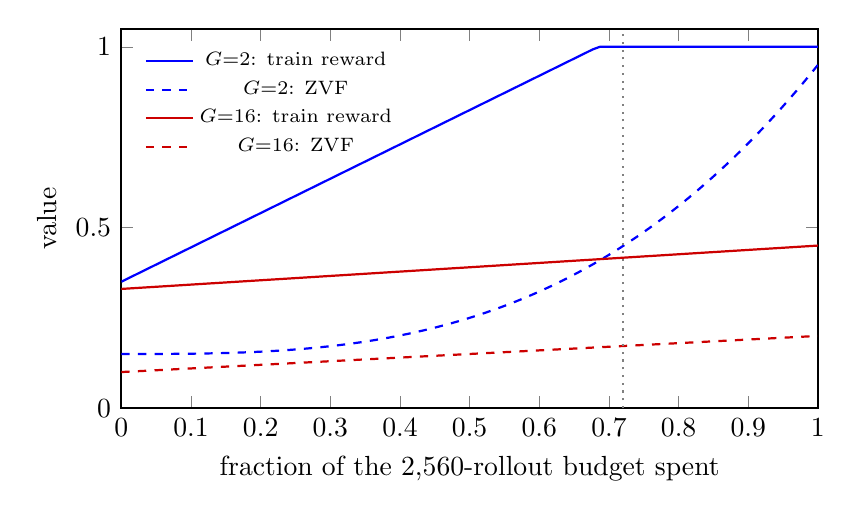
\begin{tikzpicture}
\begin{axis}[width=0.86\textwidth,height=6.4cm,
  xlabel={fraction of the 2{,}560-rollout budget spent},
  ylabel={value},
  xmin=0,xmax=1,ymin=0,ymax=1.05,
  legend style={at={(0.02,0.97)},anchor=north west,draw=none,fill=none,font=\scriptsize},
  thick]
\addplot[blue,domain=0:1,samples=100]{min(1, 0.35+0.95*x)};
  \addlegendentry{$G{=}2$: train reward}
\addplot[blue,dashed,domain=0:1,samples=100]{0.15+0.8*x^3};
  \addlegendentry{$G{=}2$: \ZVF{}}
\addplot[red!80!black,domain=0:1,samples=100]{0.33+0.12*x};
  \addlegendentry{$G{=}16$: train reward}
\addplot[red!80!black,dashed,domain=0:1,samples=100]{0.10+0.10*x};
  \addlegendentry{$G{=}16$: \ZVF{}}
\draw[gray,dotted] (axis cs:0.72,0) -- (axis cs:0.72,1.05);
\end{axis}
\end{tikzpicture}
\caption{Schematic of the measured matched-budget behaviour (Chapter~6,
seeds 123/456): the $G{=}2$ trajectory races to reward $\approx1.0$ and its
\ZVF{} climbs into the all-correct wall ($0.75$--$1.0$), while $G{=}16$
ends mid-learning ($\approx0.3$--$0.5$) with \ZVF{} low ($\le0.25$).
Right of the dotted line the $G{=}2$ reward reads success while its
gradient signal is gone. By reward alone the $G{=}2$
run looks strictly better; the (reward, \ZVF{}) pair reveals its lead
ended in zero-gradient compute.
Stylised curves; measured values in Table form in Chapter~6 and artifacts in
Appendix~B.}
\label{fig:disagreement}
\end{figure}

\section{What \ZVF{} adds over mean reward}
The sharpest demonstration comes from the matched-budget panel of Chapter~6.
Late in the $G{=}2$ arms, mean train reward sits near $1.0$ --- by the reward
axis alone, training is succeeding --- while \ZVF{} sits at $0.75$--$1.0$:
nearly every group is all-correct and contributes zero gradient. The $G{=}16$
arms at the same rollout budget hold $\ZVF\le0.25$. Reward reports \emph{where
the policy is}; \ZVF{} reports \emph{whether training is still moving}, and at
the high-accuracy end the two disagree completely. This is Claim~1 in its
purest form, and it is why the diagnostic must always be read as the pair
(reward, \ZVF{}): \ZVF{} alone aliases mastery with incapacity.

\section{The U-shape and regime aliasing}
Under binary rewards with per-prompt success rate $p$ and group size $G$, the
population zero-variance probability is the kernel $h_G(p)=p^G+(1-p)^G$ ---
a U-shape in $p$. A mean \ZVF{} therefore hides whether starvation comes from
incapacity ($p\to0$) or mastery ($p\to1$); stratified or paired-with-reward
reporting is mandatory. Empirically the observed \ZVF{} sits systematically
\emph{below} the Bernoulli-independent prediction across $G\in\{2,4,8,16\}$
(residuals $-0.13$ to $-0.23$): completions within a group are positively
informative about each other, so the contrastive signal is stronger than the
independent-coin model predicts.

\section{Diagnostic, not causal}
Two boundaries close the chapter. First, causality: \ZVF{} is a symptom
metric; interventions on it (Chapter~6) must be justified on their own
budgets, not by the correlation above. Second, telemetry robustness: the
diagnostic value of \ZVF{} depends on the reward parser's resolution
(Chapter~3), so any reported \ZVF{} must name its verifier --- one of the
reporting-standard items of Chapter~9.

% Provenance: zvf-program/theory/zvf_theory.tex (T1-T3, post-correction),
% analyze_t1_ci.py / analyze_t2_floor.py / analyze_t3_gstar.py artifacts.
\chapter{Estimation Theory and Reliability Budgets}
\label{ch:theory}

This chapter presents the theory in its \emph{corrected} form. Two errors in
the programme's earlier statements --- both found by external adversarial
review on 2026-07-11 and verified against the source --- are reported openly
in Section~\ref{sec:corrections}, because the corrections are themselves
informative.

\section{T1: \ZVF{} as a calibrated estimator}
$\ZVF_t$ over $m$ groups is an unbiased binomial-proportion estimator of the
population uniformity rate $\theta_G=\mathbb{E}_\phi[h_G(p)]$, with
$h_G(p)=p^G+(1-p)^G$ and $\phi$ the prompt-difficulty prior. Empirical
coverage on 512-prompt pools: the Wald interval covers 0.92--0.97 at
$m\ge64$ (marginal at $m{=}32$); the \textbf{Wilson interval covers
0.95--0.98 in every tested setting} and is adopted operationally.
Under difficulty-\emph{sorted} (curriculum) batching, global coverage
collapses to 0.08--0.40 --- but the interval remains calibrated (0.944) for
the \emph{local}, curriculum-stage \ZVF{}, and stratified batch composition
restores conservative global validity (0.996). The across-group-independence
threat is thus an estimand-labelling requirement, not an invalidation: report
\emph{which} \ZVF{} the interval covers.

\section{T2: the waiting-time reliability budget}
With i.i.d.\ groups, each uninformative with probability \ZVF{}, the number of
groups to the first informative one is geometric, giving
\[
N(\ZVF) \;=\; G\left\lceil \frac{\ln \delta}{\ln \ZVF}\right\rceil
\]
as the $(1{-}\delta)$-quantile of rollouts-to-first-informative-group.
\textbf{This is a reliability budget, not an impossibility bound}: an
informative group arrives within the first $G$ rollouts with probability
$1-\ZVF$, which can be large; a budget below $N$ does not make a gradient
improbable, it makes the \emph{guarantee} of one unavailable at confidence
$1-\delta$. Empirically the geometric model is essentially exact: with
$G{=}8$, $\delta{=}0.1$, the model quantile matched the observed quantile at
ratio $1.00$ in all six difficulty strata; in the hardest stratum
($\hat p\approx0.01$, $\ZVF{=}0.886$) the budget is 160 rollouts. Composed
with T1, the one-sided lower confidence bound $\underline{\ZVF}_t$ yields a
per-step, observation-driven budget $N(\underline{\ZVF}_t)$ --- conservative,
since $N$ is increasing and $N(\underline{\ZVF}_t)\le N(\ZVF_t)$.

\section{T3: the optimal group size is universal (a negative result)}
The signal-per-rollout objective
$J(G)=\tfrac1G\,\mathbb{E}_{p\sim\phi}[(1-h_G(p))\,p(1-p)]$ was intended to
yield a prior-dependent optimal group size. It does not. The identities
$1-p^2-(1-p)^2=2p(1-p)$ and $1-p^3-(1-p)^3=3p(1-p)$ hold pointwise, so
\[
J(2)\;=\;J(3)\;=\;\mathbb{E}_{p\sim\phi}\big[(p(1-p))^2\big]
\quad\text{for every prior } \phi,
\]
and $J(G)\le J(2)$ for $G\ge4$. Hence $G^\star\in\{2,3\}$ \emph{universally}:
the objective's argmax carries no information about the data, the previously
published ``empirical argmax 2--3 agrees with theory'' validation was
algebraically guaranteed rather than a test, and any data-adaptive
group-size policy must come from a richer objective (variance-, Fisher-, or
wall-clock-aware). We report this as a negative result of independent value:
it explains why per-rollout accounting always favours tiny groups, and it
sharpens Chapter~6's message that the real trade-off is temporal (early
step-count versus endgame signal), not a static optimum.

\section{Corrections adopted from external review}
\label{sec:corrections}
(1) An earlier statement of T2 claimed ``no nonzero gradient step is possible
with fewer than $N$ rollouts except with probability $<\delta$'' --- a
quantifier error confusing a quantile with a minimum; the validation script
additionally tested the inverted inequality. Both are corrected, the analysis
was re-run (fits at ratio 1.00 unchanged), and the corollary's
confidence-direction commentary was rewritten (a lower confidence bound on
\ZVF{} gives a \emph{smaller}, conservative budget). (2) The theory draft
briefly defined $\GU_t:=\ZVF_t$, contradicting the programme-wide
$\GU=1-\ZVF$; fixed. The proof-gap registers of the source paper (mixture
versus fixed-$p$ geometric modelling; improvement versus nonzero-gradient;
the global $G\ge4$ inequality) remain open and are inherited here as stated
limitations.

% Provenance: paper_P3_group_size (contrast density, Wu pairing, bridge-to-DPO
% remnant), paper_P7_zvf_controller (controller, design rules), E-R2b artifacts
% (er2b_*.json), group_size.tex + group_size_reconcile.
\chapter{Group Size as a Schedule}
\label{ch:groupsize}

\section{Static sweeps are inconclusive}
A single-seed sweep over $G\in\{2,4,8,16,32\}$ on Qwen3-8B/GSM8K is
non-monotone in fixed-step last-10 reward ($G{=}4{:}0.52$, $G{=}32{:}0.44$,
$G{=}16{:}0.38$, $G{=}2{:}0.38$, $G{=}8{:}0.34$), and a token-budget-normalised
reanalysis shifts the apparent optimum rightward with total tokens (toward
$G\approx32$ at $T\ge16$M tokens). Neither view supports a universal winner;
the honest summary is that fixed-$G$ comparisons are confounded by what the
budget is held constant \emph{in}.

\section{The matched-budget experiment (Claim 2)}
The decisive design holds the \emph{rollout budget} fixed at 2{,}560 rollouts
per arm: $G{=}2\times160$ optimiser steps versus $G{=}16\times20$ steps
(batch 8, 512-token completions, LoRA rank 4, seeds 123 and 456):
\begin{center}
\begin{tabular}{@{}lcc@{}}
\toprule
 & $G{=}2\times160$ & $G{=}16\times20$ \\
\midrule
final train reward & $\approx 0.9$--$1.0$ (pool mastered) & $\approx 0.3$--$0.5$ (mid-learning) \\
late-run \ZVF{} & $0.75$--$1.0$ (all-correct wall) & $0.00$--$0.25$ \\
late-run gradient signal & effectively zero & sustained \\
\bottomrule
\end{tabular}
\end{center}
By the reward axis alone the $G{=}2$ arms win outright --- which is exactly
the trap: their final steps are spent on zero-gradient groups.
Small $G$ converts the budget into more optimiser steps early --- consistent
with the per-rollout accounting of Chapter~5 --- and then exhausts its own
signal as accuracy rises: the $p\to1$ wall of $h_G(p)$. Large $G$ pays for
contrast it does not need early and retains signal late. \textbf{Group size
controls which end of training starves; it is a schedule variable.}

\section{Relation to the contrastive reading of GRPO}
The $G{=}2$ versus $G{=}16$ pairing is exactly the pairing behind the
``GRPO is secretly contrastive/DPO-like'' equivalence claims. Our direct test
of the generalised claim ($G{=}4\sim G{=}32$) shows retention of the large-$G$
arm's accuracy falling from $97.6\%$ at $T{=}1$M tokens to $72.7\%$ at
$T{=}64$M: the equivalence holds only in the under-trained regime. The
matched-budget panel adds the trajectory view: at a fixed rollout budget the
small-$G$ arm can even \emph{lead} on train reward, but the equivalence
claims say nothing about signal availability --- and that is where the
small-$G$ lead dies. The fuller
bridge-to-DPO treatment from the group-size working paper remains
thesis-external future work.

\begin{figure}[t]
\centering
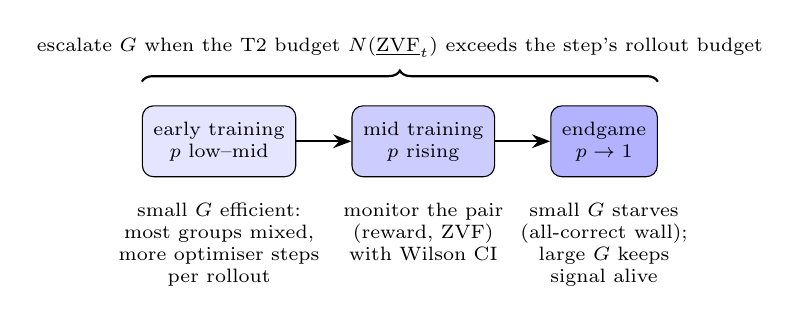
\begin{tikzpicture}[node distance=5mm and 7mm,
  stage/.style={rectangle,rounded corners,draw,align=center,minimum height=9mm,
                font=\scriptsize,inner sep=4pt},
  lab/.style={font=\scriptsize,align=center}]
\node[stage,fill=blue!10]  (early) {early training\\$p$ low--mid};
\node[stage,fill=blue!20,right=of early]  (mid) {mid training\\$p$ rising};
\node[stage,fill=blue!30,right=of mid]    (late) {endgame\\$p\to1$};
\node[lab,below=2mm of early] {small $G$ efficient:\\most groups mixed,\\
  more optimiser steps\\per rollout};
\node[lab,below=2mm of mid] {monitor the pair\\(reward, \ZVF{})\\with Wilson CI};
\node[lab,below=2mm of late] {small $G$ starves\\(all-correct wall);\\
  large $G$ keeps\\signal alive};
\draw[-{Stealth},thick] (early) -- (mid);
\draw[-{Stealth},thick] (mid) -- (late);
\draw[decorate,decoration={brace,amplitude=4pt},thick]
  ([yshift=3mm]early.north west) -- ([yshift=3mm]late.north east)
  node[midway,above=5pt,font=\scriptsize]
  {escalate $G$ when the T2 budget $N(\underline{\ZVF}_t)$ exceeds the step's
   rollout budget};
\end{tikzpicture}
\caption{Group size as a schedule. Per-rollout efficiency favours small $G$
early (Chapter~5); the all-correct wall punishes it late (Claim~2). The
escalation trigger comes from the T2 reliability budget, not from a
data-dependent ``optimal $G$'' --- which Chapter~5 shows does not exist under
per-rollout accounting.}
\label{fig:schedule}
\end{figure}

\section{Controller design (evidence-gapped, stated as such)}
A ZVF-triggered group-size controller follows from Chapters~4--5: measure
$\ZVF_t$ with its Wilson interval (T1); when the reliability budget
$N(\underline{\ZVF}_t)$ exceeds the step's remaining rollout budget, the step
fails to produce any informative group with probability $>\delta$ --- escalate
$G$ rather than gamble the budget (T2). Design rules from the controller
working paper carry over: gate on magnitude-aware statistics, escalate
multiplicatively in small steps, trigger on spikes rather than levels, never
compare controllers across stacks, and treat bought signal ($\ZVF{=}0$ via
dynamic sampling at ${\sim}45\%$ extra rollouts) as a purchase to be priced.
An offline bandit pilot recovers $97\%$ of a static oracle's informative
groups per 1{,}000 rollouts and beats uniform allocation by $28\%$.
\textbf{No efficacy claim is made} (non-claim 3): the decisive test --- a
pre-registered, compute-matched comparison against static $G{=}16$ and a
reward-only schedule, at $\ge3$ seeds on held-out metrics --- is future work,
and Chapter~5's T3 result removes any pretence that the controller could
derive a data-dependent target $G$ from the current objective.

% Provenance: paper_P4_length_bias + sections/length_bias.tex (incl. scale
% extension), E-P4 corrected panel artifacts (p4uncap_*.json), cell_runner loss
% arms, min_report loss-form item.
\chapter{Loss Form and Length Bias}
\label{ch:lossform}

\section{The question}
Dr.GRPO's motivating thesis is that GRPO's per-completion normalisations bias
updates toward longer outputs --- the ``verbosity trap'': length inflates,
then reward collapses. This chapter tests for the signature at our scale with
per-step traces of mean reward and mean completion length.

\section{Short-horizon panels at 0.5B--1.5B}
On Qwen2.5-0.5B/arithmetic (40 steps, 5 seeds per loss) and
Qwen2.5-1.5B-Instruct/GSM8K-CoT (30 steps, 3 seeds per loss), neither GRPO nor
Dr.GRPO exhibits the trap: per-run $\rho(\text{step},\text{len})$ is
consistently \emph{negative} (models get shorter as training proceeds). These
runs are cap-bounded (200-token generation cap) and short-horizon; the
original Dr.GRPO evidence sits at hundreds of steps, an order of magnitude
beyond ours --- our data is consistent with the early phase of that curve.

\section{The uncapped 8B panel}
A six-arm panel extends the scale axis: Qwen3-8B, GSM8K, 30 steps, $G{=}8$,
batch 4, \textbf{three seeds per loss}, completion cap raised $5\times$ to
1{,}024 tokens. Results:
\begin{center}
\begin{tabular}{@{}lccc@{}}
\toprule
arm & len first-5 $\to$ last-10 & late \ZVF{} & late reward\\
\midrule
GRPO s42/s123/s456 & $1004{\to}905$, $981{\to}944$, $996{\to}900$ &
$0.47$, $0.47$, $0.55$ & $0.75$, $0.68$, $0.76$\\
Dr.GRPO s42/s123/s456 & $999{\to}931$, $972{\to}902$, $1000{\to}878$ &
$0.45$, $0.72$, $0.70$ & $0.74$, $0.78$, $0.78$\\
\bottomrule
\end{tabular}
\end{center}
\textbf{No length inflation in either loss} --- all six arms shrink 6--12\%
--- and \textbf{no late-\ZVF{} separation} between the losses. Step-0 lengths
sit near the raised cap ($\approx98\%$), so upward headroom remains limited,
but trajectories move \emph{away} from the cap, so the compression finding is
not a censoring artifact. The 30-step horizon caveat stands.

\section{Provenance: this panel was run twice}
The first version of this panel was \emph{invalid}: the runner's
\texttt{--loss drgrpo} flag was documented (its commit message claimed the
mapping) but never wired to the advantage normalisation, so both ``arms''
silently trained vanilla GRPO --- and no reward, length, or \ZVF{} trace
revealed it. The defect was caught only by reading the runner. The invalid
artifacts are preserved under explicit \texttt{.invalid\_actually\_grpo.json}
names; the corrected rerun (same day) produced the table above, and notably
\emph{reversed} the invalid panel's secondary claim (the invalid data had
suggested Dr.GRPO keeps more groups live; the corrected data shows
equal-or-higher late \ZVF{} for Dr.GRPO). Chapter~9 turns this incident into
protocol.

\section{Conclusion of the chapter}
At the scales and horizons this programme can afford, the loss-form choice
between GRPO and Dr.GRPO has no observable footprint on length or \ZVF{}.
This is evidence about \emph{reporting} rather than about superiority: a
comparison between these losses at this scale measures noise unless the stack
is controlled far more tightly than the labels suggest.

% Provenance: paper_P1_scaling (demoted from "law" to observations),
% MATH-500/MBPP panels, frontier synthesis sections, pass@k protocol.
\chapter{Scaling and Transfer Observations}
\label{ch:scaling}

\section{Scope discipline}
The programme's cross-library corpus (70+ logged runs, seven libraries, five
model families, 0.6B--671B) supports \emph{observations}, not laws: most cells
are single-seed, backends differ, and the term ``scaling law'' is deliberately
avoided (external review, Chapter~9). The full scaling-law treatment of the
corresponding working paper is demoted to this observational chapter.

\section{What the corpus shows}
Model scale does not uniformly reduce \ZVF{} ($r\approx-0.26$ across logged
runs), and after accounting for task type, model family alone does not explain
performance variance (one-way ANOVA $F(4,10){=}0.949$, $p{=}0.476$). The
practical reading: signal starvation is a property of the (task difficulty
$\times$ group size $\times$ training phase) geometry, not something scale
buys you out of.

\section{Transfer and difficulty extension}
Post-RL adapters trained on GSM8K show \emph{zero forgetting and mild positive
transfer} on MBPP (pass@32, all adapters within noise of or above base across
$G\in\{2,4,16,32\}$). On the matched base-versus-post-RL pass@$k$ panel,
pass@1 deltas scatter from $-0.5$ to $+1.9$ points --- under pass@1-only
reporting the $G{=}2$ arm would read as a regression --- while the pass@32
frontier improves $+1.5$ to $+2.5$ points in all four arms; none of this
reaches significance at a single training seed, which is exactly why pass@$k$
curves with stated noise bands are a reporting-standard item (Chapter~9).
On MATH-500, the harder-task extension, the base-model panel is complete and
the post-RL panels are partial at the time of writing; the partial result is
that \textbf{GSM8K-trained gains do not replicate on hard math} --- the
frontier shift observed on GSM8K-family tasks does not carry, reinforcing the
distribution-sharpening (rather than capability-expansion) interpretation and
the thesis's non-claim~4.

\section{Takeaway}
Scaling observations here serve one purpose: bounding the claims. The
capability headroom analysis (pass@32 $=91\%$ on GSM8K), the non-transfer to
MATH-500, and the single-seed density of the cross-scale corpus jointly
justify why Claims~1--2 are stated at the stack level and nowhere above it.

% Provenance: paper_P5_minreport (eight-item standard, threat model, toolchain),
% paper_P6_registry, zvf-program position + registry drafts, reproducibility_audit
% (survival protocol, as future work), loss-flag incident, audit rounds 2026-07-11.
\chapter{Reproducibility: Standard, Registry, and a Case Study}
\label{ch:repro}

\section{The thesis of this chapter}
An algorithm \emph{label} underdetermines the executed update rule. Measured
instances from this programme: swapping the training backend under a fixed
label --- which, undisclosed, also bundled a different base checkpoint ---
moved final reward across a $17\times$ span ($85.6\%$ versus $5.0\%$); the
same ``DAPO'' label yielded mean \ZVF{} $0.00$ on an open trainer with true
dynamic sampling but $0.58$ on a closed stack running an asymmetric-clip
surrogate; and a sub-resolution reward jitter collapsed batch \ZVF{}
$0.158\to0.000$. Stack identity cannot be certified from plausible-looking
outputs; it must be certified from the stack.

\section{Case study: the unwired loss flag}
On 2026-07-11 this programme shipped exactly the failure its standard targets.
A six-arm GRPO-versus-Dr.GRPO panel ran with a \texttt{--loss drgrpo} flag
whose commit message claimed it toggled the advantage normalisation; the flag
was never wired. Both arms silently trained the identical objective under two
labels. No output-level trace --- reward, length, \ZVF{} --- revealed it; the
defect was found only by reading the runner. Response protocol, now standard
practice here: invalidate loudly (artifacts preserved under
\texttt{.invalid\_actually\_grpo.json} names), fix, rerun the same day, and
record that the corrected panel \emph{reversed} one of the invalid panel's
conclusions (Chapter~7). Two subsequent whole-repository adversarial audits
(one human-directed multi-model review; one file-grounded frontier-model pass)
surfaced and led to fixes for: two theory statement errors (Chapter~5), an
inverted validation inequality, a systematic off-by-one in seven training
scripts (a spurious token-0 target at every sequence end), uncontrolled
generation seeds, an over-permissive reward parser, and a Monte-Carlo
``truth'' treated as exact. A third audit pass produced only fabricated
findings (invented file paths and quotes), all refuted against the source ---
itself a demonstration that \emph{plausible-but-wrong survives until verified
against the stack}.

\section{The eight-item minimum reportable stack}
Every item earns its place via a documented lever from this corpus:
(1) loss form (ratio level, clip, mask, normalisation, dynamic-sampling
status); (2) reference policy and KL handling; (3) sampler/backend/precision
\emph{including base-checkpoint identity}; (4) per-step \ZVF{}/\GU{}
trajectory; (5) group-size schedule; (6) held-out split disjoint from the
reward environment; (7) decontamination and a parser-robustness probe;
(8) held-out pass@$k$ curves alongside pass@1, with temperature and completion
budget. Items are checkable; a manifest emitter and a 0--100 auditor badge
ship with the bench.

\section{The registry}
A machine-readable registry records stacks and variant deltas: a JSON schema
embedding the eight-item block, variant-delta records verified against the
DAPO/Dr.GRPO/GSPO papers, twenty seed stack entries, and \texttt{stackdiff},
which maps a pair of entries to a flip-risk verdict (R0--R5) --- flagging, for
example, the open-versus-closed ``DAPO'' pair above as an R5 label-flip risk
from manifests alone. Where measured evidence exists it is tiered; the
Dr.GRPO delta carries two measured panels (Chapter~7) showing no length or
\ZVF{} footprint at this scale, against its registry-claimed sign.

\section{The survival audit (future work, gated)}
The natural enforcement instrument --- re-implement DAPO, GSPO, Dr.GRPO, and
MAD-GRPO in one controlled stack and measure which claimed gains survive ---
is specified but \emph{deliberately deferred}: a programme weeks past its own
silent-equivalence incident lacks standing to adjudicate others'
implementations. Gates before execution: an open stack (not a closed managed
API), differential-objective test tooling that would have caught the loss-flag
bug automatically, and one method at a time. This ordering --- earn
credibility, then audit --- is itself a finding of the external reviews.

\section{On AI-assisted drafting}
The seventeen working papers behind this thesis were drafted with heavy
agent assistance against real measured artifacts. The audit trail of this
chapter is the honest account of what that workflow produced: real
measurement at unusual volume, real defects at unusual volume, and a
verification discipline as the only thing separating the two. Every number in
this thesis survived the audits or was corrected by them, with both states
recorded in version control.

% Provenance: consolidation plan v3, advisor brief, review verdicts.
\chapter{Conclusions, Limitations, and Future Work}
\label{ch:conclusion}

\section{What this thesis established}
Under binary verifiable rewards, group-relative training starves at both ends
of the difficulty spectrum, and the Zero-Variance Fraction --- read jointly
with mean reward --- is a near-free, calibrated instrument that sees both
walls, including the one reward curves cannot show (Claim~1). Group size
selects which wall a fixed rollout budget hits: small $G$ buys early optimiser
steps and starves in the endgame; large $G$ holds signal throughout
(Claim~2). The estimation theory supporting the instrument is calibrated
(Wilson CIs), its waiting-time budget is empirically exact at ratio 1.00, and
its would-be optimal-group-size theory resolves to an honest negative result:
per-rollout accounting always answers $G^\star\in\{2,3\}$, for any data, so
adaptivity must be justified by richer objectives.

\section{Limitations}
All training-side evidence sits on one model (Qwen3-8B, LoRA rank 4), one
task family (GSM8K, binary rewards), one managed API with a closed loss
kernel, at 1--3 seeds per result; pre-2026-07-11 artifacts additionally carry
a since-fixed off-by-one target and v1 parser semantics. \ZVF{} as defined is
specific to (near-)discrete rewards; continuous-reward analogues (e.g.\
contrast-density statistics) are sketched but not validated. The pooled
cross-scale correlations are descriptive only. Theory carries declared proof
gaps. None of the seventeen working papers is submission-ready as a standalone
unit --- by design, after external review (below).

\section{Publication roadmap (post-degree, gated)}
Following three rounds of external review, the programme's publication plan
is thesis-first: (i) a bounded diagnostic paper (Claims~1--2, this thesis's
Chapters~4--6 core) is publishable without any controller claim; (ii) the
controller paper is gated on a pre-registered, compute-matched win over
static $G{=}16$ \emph{and} a reward-only schedule at $\ge3$ seeds;
(iii) the survival audit is gated on an open stack and differential-objective
test tooling; (iv) the benchmark remains a versioned artifact. The
seventeen-document corpus maps onto these vehicles and this thesis per
Appendix~A.

\section{Future work}
Beyond the gates above: MATH-500 and code-task completion of the capability
panels; a clustered-variance CI for curriculum-ordered training; a
variance-aware replacement for the T3 objective; continuous-reward \ZVF{}
analogues; and the full bridge-to-DPO analysis of the group-size working
paper.

\section{Closing}
The programme's most transferable lesson is methodological: at this scale,
the binding constraint on RL post-training research is not compute or
algorithmic novelty but \emph{certainty about what actually ran}. A cheap
diagnostic that cannot be gamed by a pretty reward curve, a reporting standard
whose every item once flipped a result, and the habit of reading the runner
--- these travelled further than any single number in this thesis.


\appendix
\chapter{Provenance: the Seventeen Working Papers}
\label{app:papermap}

This thesis consolidates seventeen working documents produced during the
programme. Each row names the document, its repository path, and the chapter
that absorbs its content. Canonicalisation decisions (which drafts are
authoritative where they overlap) follow the reviewed consolidation plan in
\texttt{platform\_hybrid/paper/PAPERS\_README.md}.

\begin{center}
\small
\resizebox{\textwidth}{!}{%
\begin{tabular}{@{}rp{5.6cm}p{9.0cm}l@{}}
\toprule
\# & Document & Path (repo-relative) & Absorbed by\\
\midrule
1 & Unified benchmark paper & \texttt{platform\_hybrid/paper/main.tex} & Ch.~3\\
2 & ACM reformat of \#1 & \texttt{platform\_hybrid/paper/acm\_main.tex} & Ch.~3\\
3 & Workshop variant & \texttt{...{/}neurips\_2026\_variants/main\_workshop.tex} & Ch.~3, 6\\
4 & ZVF stratified audit & \texttt{...{/}neurips\_2026\_variants/main\_zvf.tex} & Ch.~4\\
5 & Reproducible-artifact variant & \texttt{...{/}neurips\_2026\_variants/main\_dnb.tex} & Ch.~3, 9\\
6 & P1 scaling laws & \texttt{platform\_hybrid/paper/paper\_P1\_scaling.tex} & Ch.~8\\
7 & P2 ZVF diagnostic & \texttt{...{/}paper\_P2\_zvf.tex} & Ch.~4\\
8 & P3 group size / DPO bridge & \texttt{...{/}paper\_P3\_group\_size.tex} & Ch.~6\\
9 & P4 length bias & \texttt{...{/}paper\_P4\_length\_bias.tex} & Ch.~7\\
10 & P5 MIN-REPORT-RL & \texttt{...{/}paper\_P5\_minreport.tex} & Ch.~9\\
11 & P6 GRPO-Registry & \texttt{...{/}paper\_P6\_registry.tex} & Ch.~9\\
12 & P7 ZVF controller & \texttt{...{/}paper\_P7\_zvf\_controller.tex} & Ch.~6\\
13 & P8 fraud detection & \texttt{...{/}paper\_P8\_fraud.tex} & out of programme$^\ast$\\
14 & ZVF theory (T1--T3) & \texttt{zvf-program/theory/zvf\_theory.tex} & Ch.~5\\
15 & MIN-REPORT position draft & \texttt{zvf-program/position/min\_report\_rl.tex} & Ch.~9\\
16 & Registry living catalog & \texttt{zvf-program/registry/grpo\_registry.tex} & Ch.~9\\
17 & Survival audit protocol & \texttt{zvf-program/audit/reproducibility\_audit.tex} & Ch.~9 (future work)\\
\bottomrule
\end{tabular}}
\end{center}

\noindent$^\ast$Document 13 concerns an unrelated fraud-detection domain; it
is excluded from this thesis's claims and retained in the repository as an
independent working paper. Its absorption here consists of this provenance
entry and the consolidation decision that removed it from the programme.

Documents 2 and 3 are venue reformats of document 1 and are absorbed
transitively. Where documents 10/15, 11/16, and 12/14 overlap, the
canonicalisation notes embedded in each source file identify the
authoritative draft; this thesis reflects the post-merge, post-correction
state of 2026-07-12.

\chapter{Claim-to-Artifact Map}
\label{app:artifacts}

Every quantitative claim in this thesis traces to a version-controlled
artifact in \texttt{arvindcr4/tinker-rl-lab} (result JSONs; W\&B mirrors in
the \texttt{zvf-training}, \texttt{zvf-experiments-next}, and
\texttt{modal-open-stack} projects).

\begin{center}
\small
\begin{tabular}{@{}p{6.2cm}p{7.2cm}@{}}
\toprule
Claim / number & Primary artifact(s)\\
\midrule
GSM8K base pass@\{1,8,32\} $=30.4/79.7/91.0\%$ &
\texttt{experiments-next/results/passk\_qwen3-8b\_base\_test\_p200\_n32\_s42.json}\\
Train-pool rollout quality (\ZVF{} $10.86\%$ etc.) &
\texttt{quality\_pool\_qwen3-8b\_train\_n512\_r32\_s42.json}\\
T1 coverage (Wilson $0.95$--$0.98$; curriculum collapse) &
\texttt{t1\_ci\_coverage\_*.json}, \texttt{analyze\_t1\_ci.py}\\
T2 quantile fit (ratio $1.00$, six strata; 160-rollout budget) &
\texttt{t2\_floor\_qwen3-8b\_train\_n512\_r32\_s42\_G8.json} (corrected check)\\
T3 universality ($J(2){=}J(3)$) &
\texttt{zvf\_theory.tex} eq.~(J23); \texttt{analyze\_t3\_gstar.py}\\
Claim 2 matched-budget panel (E-R2b) &
\texttt{tinker-runs/results/er2b\_\{g2,g16\}\_s\{123,456\}.json}\\
Loss-form panel (E-P4, corrected; 6 arms) &
\texttt{tinker-runs/results/p4uncap\_\{grpo,drgrpo\}\_s\{42,123,456\}.json}\\
Invalid first panel (preserved) &
\texttt{p4uncap\_drgrpo\_*.invalid\_actually\_grpo.json}\\
MBPP transfer; base-vs-post-RL pass@$k$ frontier &
\texttt{passk\_lightning\_*.json}, \texttt{passk\_colab\_*.json}\\
MATH-500 non-replication (partial) &
\texttt{passk\_modal\_*math500*.json}\\
Backend $17\times$ span; ``DAPO'' \ZVF{} $0.00$ vs $0.55$--$0.58$ &
cross-stack audit artifacts (registry seed entries)\\
Parser micro-jitter probe ($0.158\to0.000$) &
convergent-repository experiment records (P5 evidence)\\
Loss-flag incident timeline &
commits \texttt{4847764}, \texttt{1959eff}, \texttt{212ff0e}; fleet logs\\
Audit-round fixes (2026-07-11) &
commits \texttt{5486ae2}, \texttt{acc08eb}\\
\bottomrule
\end{tabular}
\end{center}

\paragraph{Reproduction.} \texttt{REPRODUCE.md} at the repository root
documents environment setup; the experiments-next suite is offline-resampled
from committed pools wherever possible, so the T1/T2/T3 analyses re-run
without API credits. Training reruns require Tinker credits and are
checkpointed/resumable (Chapter~3).


\end{document}
